% Performance evaluation
% Benchmark de Dani
% Robar algo de la tesis de Dani para comentar sobre el benchmark?
% Comparación con la versión previa
% Gráficos dcs vs dcs 2, dcs2 vs las otras herramientas

Para realizar las pruebas de performance decidimos utilizar el mismo conjunto de problemas creado y utilizado en \cite{tesisDani} para examinar el algoritmo original de $DCS$, ya que nuestra intención era principalmente compararnos contra la versión anterior. En esta sección presentamos los resultados de la comparación versus dicha versión y, además, contra diversos programas del estado del arte de resolución de problemas de síntesis.

Todos los casos de estudios fueron escritos de manera de poder modificar el número de componentes y estados, con la intención de probar escalabilidad dentro de cada tipo de problema.
\begin{description}
    \item [Transfer Line] Automatización de una fabrica, un dominio de mucho interés en el área de supervisory control. TL consiste de n máquinas conectadas por $n$ buffers cada uno con capacidad de $k$ unidades, termina en una máquina adicional llamada Test Unit.
    
    \item [Dinning Philosophers] Problema clásico de concurrencia. En DP hay $n$ filósofos sentados en una mesa redonda, cada uno comparte un tenedor con sus vecinos aledaños. El objetivo del sistema es controlar el acceso a los tenedores de manera que los filósofos puedan alternar entre comer y pensar; evitando \textit{deadlock} y \textit{starvation}. Adicionalmente, cada filósofo, luego de tomar un tenedor, debe cumpplir con $k$ pasos de etiqueta antes de comer.

    \item [Cat and Mouse] Juego de dos jugadores donde cada uno toma turnos para moverse a una casilla adjacente dentro de un mapa de la forma de un corredor dividido en $2k + 1$ áreas. En CM $n$ gatos y la misma cantidad de ratones son colocados en extremos opuestos del corredor. El objetivo es mover a los ratones de manera que no terminen en el mismo lugar que un gato. Los movimientos de los gatos no son controlables. En el centro del corredor hay un agujero que lleva a los ratones a un área segura.
    
    \item [Bidding Workflow] Modela el proceso de evaluación de proyectos de una empresa. El proyecto debe ser aprobado por $n$ equipos. El objetivo es sintetizar un flujo de trabajo que intente llegar a un concenso, es decir, aprobar/rechazar el proyecto cuando todos los equipos lo aceptan/rechazan. La propuesta puede ser reasignada para re-evaluación por un equipo hasta $k$ veces, no se puede reasignar si el equipo ya lo había aceptado. Cuando un equipo lo rechaza $k$ veces el proyecto puede ser rechazado sin concenso. Es un caso de estudio típico del dominio de Business Process Management.
    
    \item [Air-Traffic Management] Representa la torre de control de un aeropuerto, que recibe $n$ peticiones de aterrizaje simultáneas. La torre necesita avisar si tiene permiso para aterrizar o, en caso contrario, en cuál de los $k$ espacios aéreos debe realizar maniobras de espera. El objetivo es que todos los aviones puedan aterrizar de manera segura. El problema solo tiene solución si la cantidad de aviones es menor a la de espacios aéreos ($n<k$).
    
    \item [Travel Agency] Modela una página on-line de ventas de paquetes de viajes. El sistema depende de $n$ servicios de terceros para realizar las reservas (ej. alquiler de auto, compra de pasajes, etc). Los protocolos para utilizar los servicios pueden variar de manera no controlable; una variante es la selección de hasta $k$ atributos (ej. destino del vuelo, clase y fechas). El objetivo del sistema es osquestar los servicios de manera de obtener un paquete de vacaciones completo de ser posible, evitando pagar por paquetes incompletos.
\end{description}

\section{Comparación con versión previa de DCS}
Como ya dijimos el principal foco del trabajo fue de brindar una mayor seguridad sobre la correctitud y completitud del approach novedoso de la exploración on the fly. Esto debía hacerse sin perder la buena performance que aportaba la técnica, con el foco de poder aplicarla a casos de mayor tamaño. Aclaramos que el benchmark se corrió en un equipo de las mismas características para ambas versiones de DCS.

La comparación se realizó para dos heurísticas distintas, $Monotonic Abstraction$ y $Ready Abstraction$, desarrolladas en \cite{tesisDani}, para observar la diferencia de performance en distintas condiciones. Puede notarse que la segunda heurística supera ampliamente a la primera, pero que para ambas las diferencias entre los algoritmos de exploración es mínima.

\begin{figure}[htb]
    \centering
    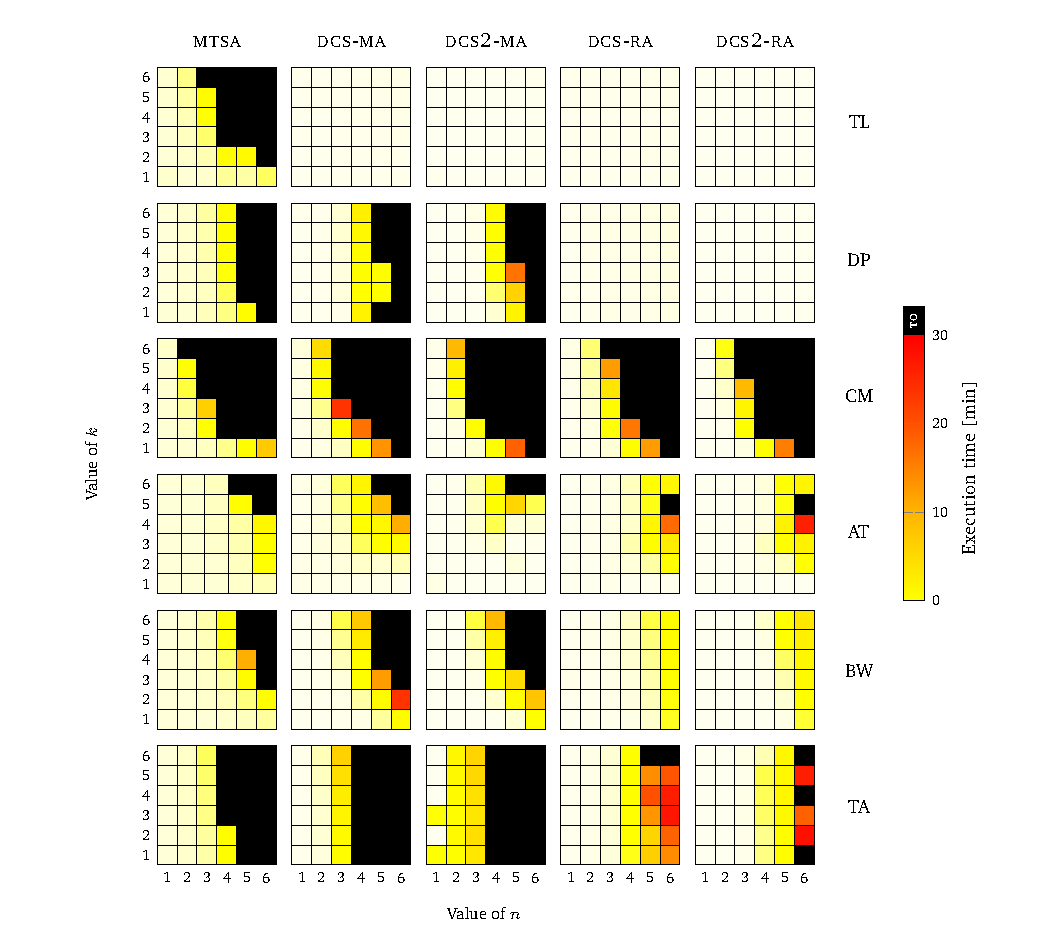
\includegraphics[width=\linewidth]{figures/dcs_vs.pdf}  
    \caption{dcs2 = performance nuevo algoritmo}
    \label{fig:dcs_vs}
\end{figure}


En la figura~\ref{fig:dcs_vs} puede verse la comparación y que en la mayoría de los problemas los resultados son similares. En los problemas $CM$ y $TA$, la nueva versión del algoritmo $DCS2$ no logra resolver algunas instancias antes del $timeout$ que previamente podían ser resueltas. No consideramos eso como una señal mayor de mala performance en el algoritmo, ya que hay otros problemas como $AT$ y $BW$ donde los resultados para la heurística $Monotonic Abstraction$ no solo no empeoraron sino que mejoraron.

Es esperable que en un proceso exploratorio guiado de forma heurística, cambios en la poda de ramas (por la clasificación o falta de la misma de ciertos estados) van a llevar a explorar caminos más o menos fructíferos según la estructura del problema. Lo relevante de la comparación es que no se observa una diferencia generalizada en los desempeños de las distintas versiones del algoritmo de exploración.

De estos resultados concluímos que las modificaciones al algoritmo no afectan de forma significativa su performance.

\section{Comparación con otros programas}

En función de la completitud del capítulo decidimos agregar los gráficos de comparación entre DCS2 y las herramientas utilizadas en \cite{tesisDani}. Al igual que su versión anterior DCS2 supera ampliamente en muchas de las instancias a las demás herramientas del estado del arte, esto se puede apreciar en la figura~\ref{fig:vs_otros}. Además la figura~\ref{fig:dcs:results} muestra un resúmen visual de total de instancias resultas y tiempo de ejecución, respectivamente.


\begin{figure}[htb]
	\centering
	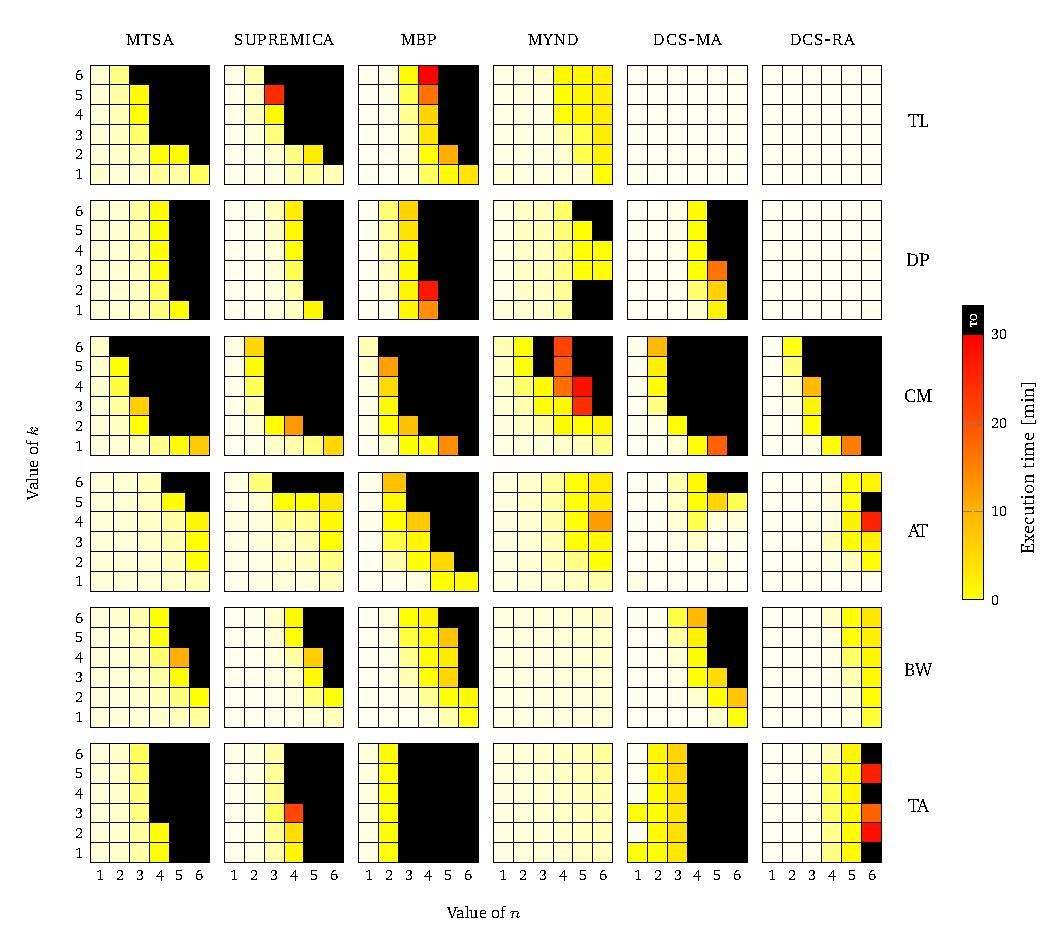
\includegraphics[width=\linewidth]{figures/nuestrosResults/detailed.pdf}  
	\caption{comparación detallada}
	\label{fig:vs_otros}
\end{figure}

\begin{figure*}[th]
	\centering
	\vspace{10cm}
	\hspace{-2cm}
	\begin{minipage}[T]{1.20\linewidth}
		\vspace{-95mm}
		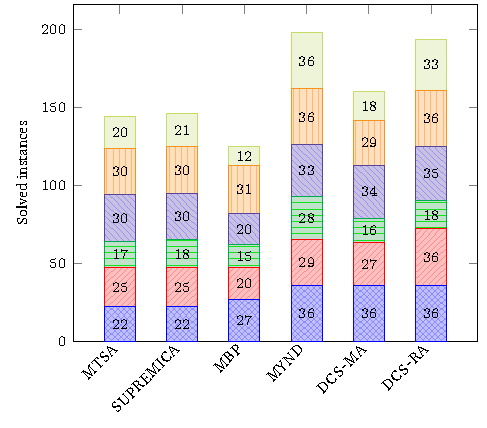
\includegraphics[scale=.905]{figures/nuestrosResults/instances.pdf}\label{fig:dcs:results:instances}
		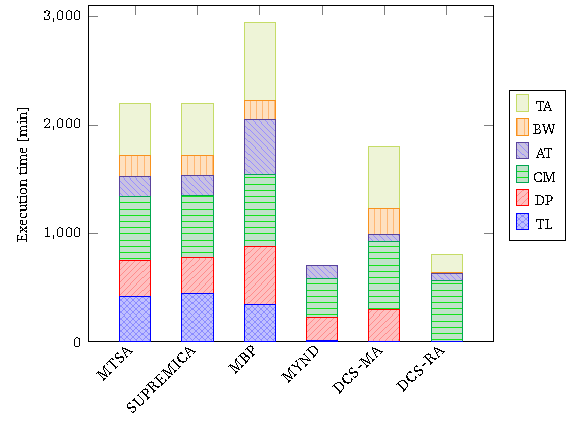
\includegraphics[scale=.905]{figures/nuestrosResults/time.pdf}\label{fig:dcs:results:time}
	\end{minipage}
	\caption{Cantidad total de instancias resueltas (izquierda) y tiempo de ejecución (derecha) con \DCS y otras herramientas.}
	\label{fig:dcs:results}
\end{figure*}










